\documentclass{article}
\usepackage{graphicx}
\usepackage{caption}
\usepackage{subcaption}
\usepackage[paper=a4paper,margin=1in]{geometry}
\usepackage[fontsize=12pt]{fontsize}
\usepackage{amsmath, amsthm, amssymb}
\usepackage[hidelinks]{hyperref}
\usepackage[nameinlink, noabbrev]{cleveref}

\newtheorem{theorem}{Theorem}[section]
\DeclareMathOperator{\sgn}{sgn}

\title{Math 475 -- Project 2 \\ Stochastic Bobcat Population}
\author{Jackson Brienen}
\date{October 17 2025}

\begin{document}

\maketitle

\section{Introduction}

In this paper we discuss how we can model bobcat populations using stochastic models. We study three different models, one being the basic exponential model, and two being different stochastic models. We approach the models with the follow assumptions:

\begin{enumerate}
    \item Any initial population, denoted $P(0)$ will be greater than zero, usually $P(0)=100$.
    \item There is no carrying capacity/ maximum population.
    \item All births and deaths happen at the end of a year/ start of a new year.
    \item All time increments, denoted $t$, are integers greater than or equal to zero.
    \item We assume, in most cases, that fractional populations are valid.
\end{enumerate}

This paper is divided into four main topics. First, a review of the standard exponential population model. Next, a look a demographic stochasticity, i.e. variability in internal growth rates. Then, we look at environmental stochasticity, which is variability in external factors which will affect population growth. Finally, we look at model which combines both environmental and demographic stochasticity.

\section{Exponential Model}

The basic exponential model for bobcat population usually written as \cref{eq:exponential-basic}, focuses primarily on a growth rate $r$. We can expand this parameter to be more realistic, including a birth rate, $b$, and survival rate, $s$. Where $1 + r = b + s$, this creates the more realistic model in \cref{eq:exponential}.

\begin{equation} \label{eq:exponential-basic}
    P(t) = (1 + r)P(t-1)
\end{equation}

\begin{equation} \label{eq:exponential}
    P(t) = (b+s)P(t-1)
\end{equation}

We know that this recurrence simplifies to the exponential function $(r + 1)^tP(0)$, and with our added parameters $(b + s)^tP(0)$. We see this exponential nature in \cref{fig:exponential}. Furthermore, we also see the expected exponential growth as if $b=0.4$ and $s=0.68$, then $s+b = 1.08$. This is the equivalent of having $r = 0.08$ in our simpler formula, which is a positive growth rate.

\begin{figure}
    \centering
    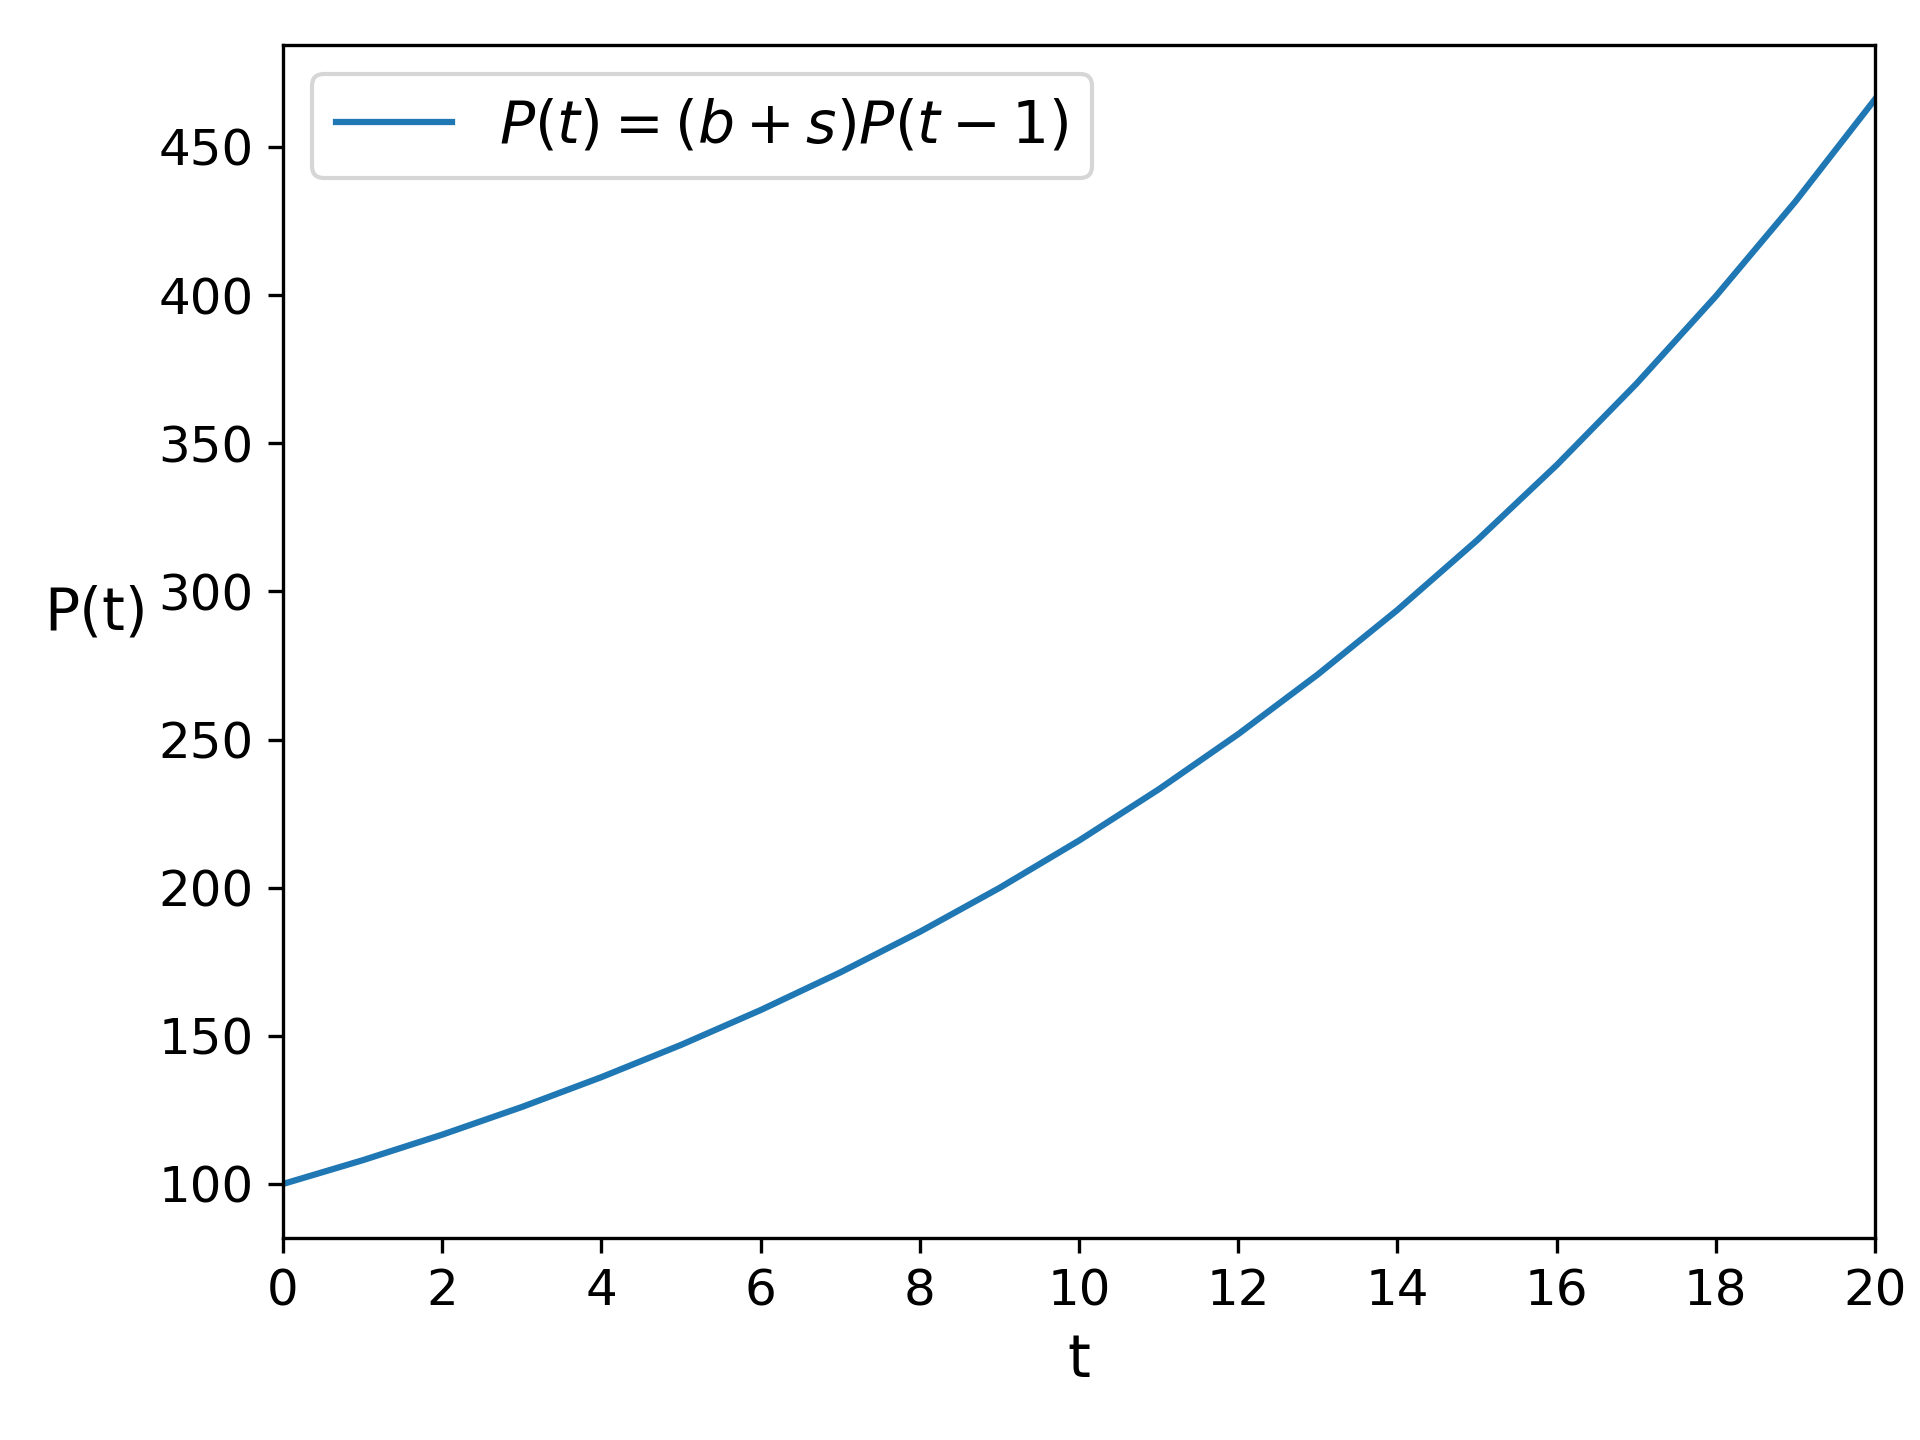
\includegraphics[width=.5\linewidth]{plots/exponential.png}
    \caption{Bobcat population over 20 years with an initial population $P(0)=100$, birth rate $b=0.4$, and survival rate $s=0.68$.}
    \label{fig:exponential}
\end{figure}

\section{Demographic Stochasticity}
While the basic exponential model gives us a good start, it is not very realistic. A constant birth and death rate is unlikely to happen in real life, so we can attempt to mimic this using demographic stochasticity. Previously our model was deterministic, i.e. the results that we see in \cref{fig:exponential} with the given parameters, will always be the results for those parameters. In a stochastic the model will have parameters that rely on randomness, so using the same model twice may give different results.

For demographic stochasticity we introduce randomness on the two internal parameters, the birth and survival rates. To introduce this randomness we will use a normal distribution. Commonly denoted $z \sim \mathcal{N}(\mu, \sigma)$, where $\mu$ is the mean and $\sigma$ is the standard deviation. The formula for the probability density, seen in \cref{eq:standard-distribution}, describes the general likelihood of a given value, $x$, being chosen.

\begin{equation} \label{eq:standard-distribution}
    f(x) = \frac{1}{\sigma\sqrt{2\pi}}e^{-\frac{1}{2}\left(\frac{x-\mu}{\sigma}\right)^2}
\end{equation}

\begin{figure}[h!]
    \centering
    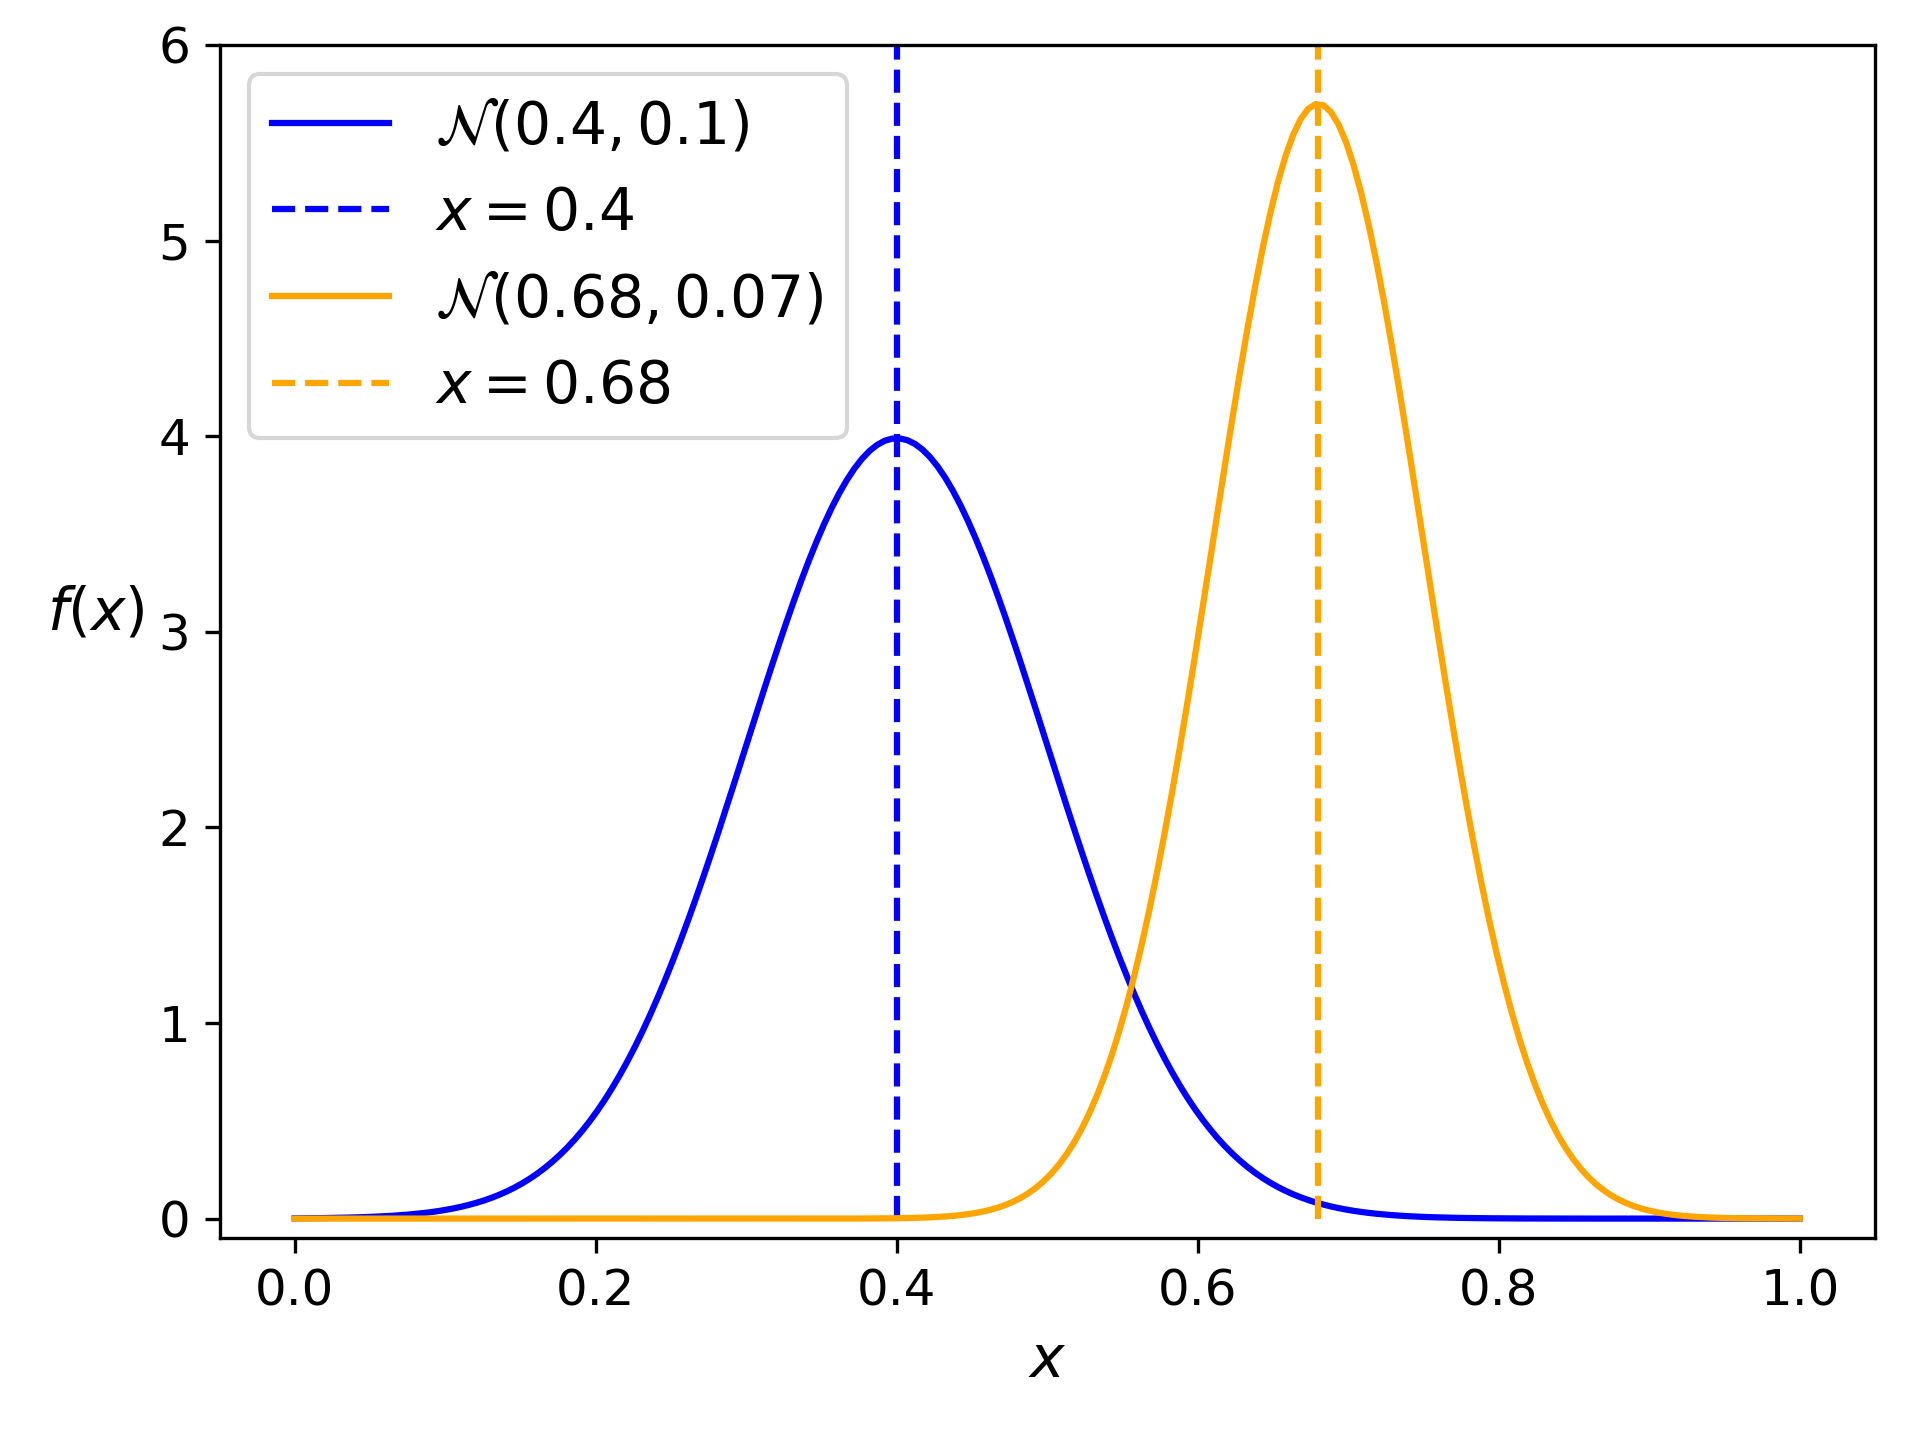
\includegraphics[width=.5\linewidth]{plots/standard-distribution.png}
    \caption{Probability density of standard distributions with means of 0.4 and 0.68, and standard deviations 0.1 and 0.07.}
    \label{fig:standard-distribution}
\end{figure}

Looking at the standard distribution probability densities in \cref{fig:standard-distribution}, we can get a sense of that the standard distribution does. The area under any given region of a curve is the percent chance for those values to be picked, while the area under the whole curve will always be 1 (100\%), provided $\sigma > 0$. In \cref{fig:standard-distribution} we plot $\mathcal{N}(0.4, 0.1)$, the blue line, and $\mathcal{N}(0.68, 0.07)$, the orange line, which will be the distributions we will use for our $b$ and $s$ parameters respectively.

When analyzing this model, due to its inherent randomness, we must take multiple samples or trial runs. We will analyze three components of the model, the maximum population produced, the minimum population produced, and the median population produced. We will compare each of these to the standard deterministic model. It does not make sense to analyze the average population produced by the model. Due to how the normal distribution works, as trial runs increase, the closer the model's average will get to the deterministic model regardless of the standard deviation for the two parameters.

\begin{figure}[h]
    \centering
    \begin{subfigure}{.5\textwidth}
        \centering
        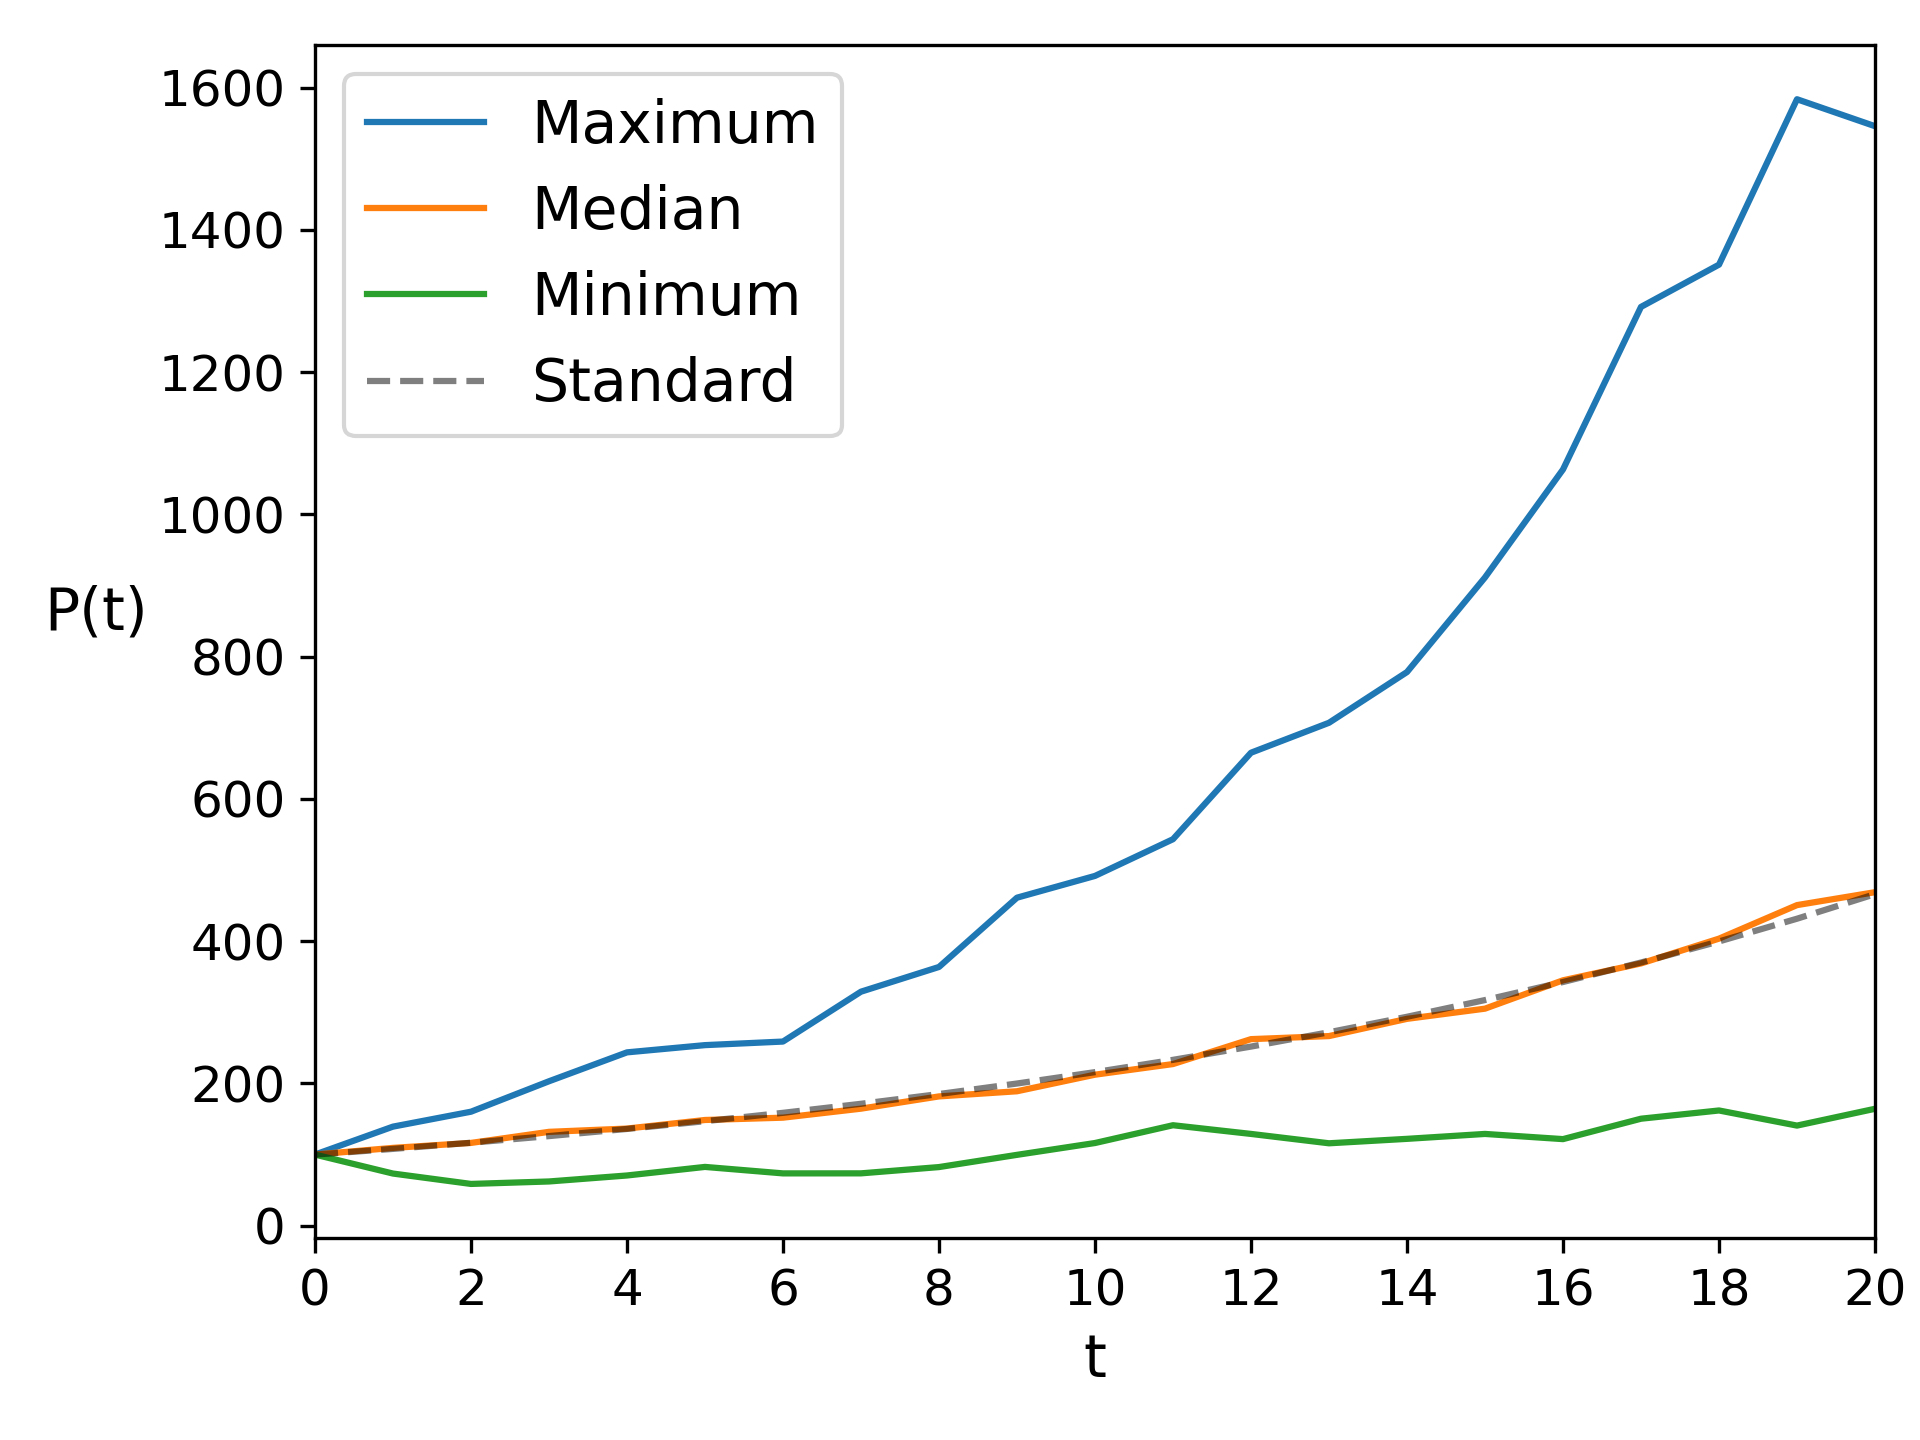
\includegraphics[width=.95\linewidth]{./plots/demographic.png}
        \caption{$b = \mathcal{N}(0.4,0.1)$ and $s = \mathcal{N}(0.68, 0.07)$}
        \label{fig:demographic-standard}
    \end{subfigure}%
    \begin{subfigure}{.5\textwidth}
        \centering
        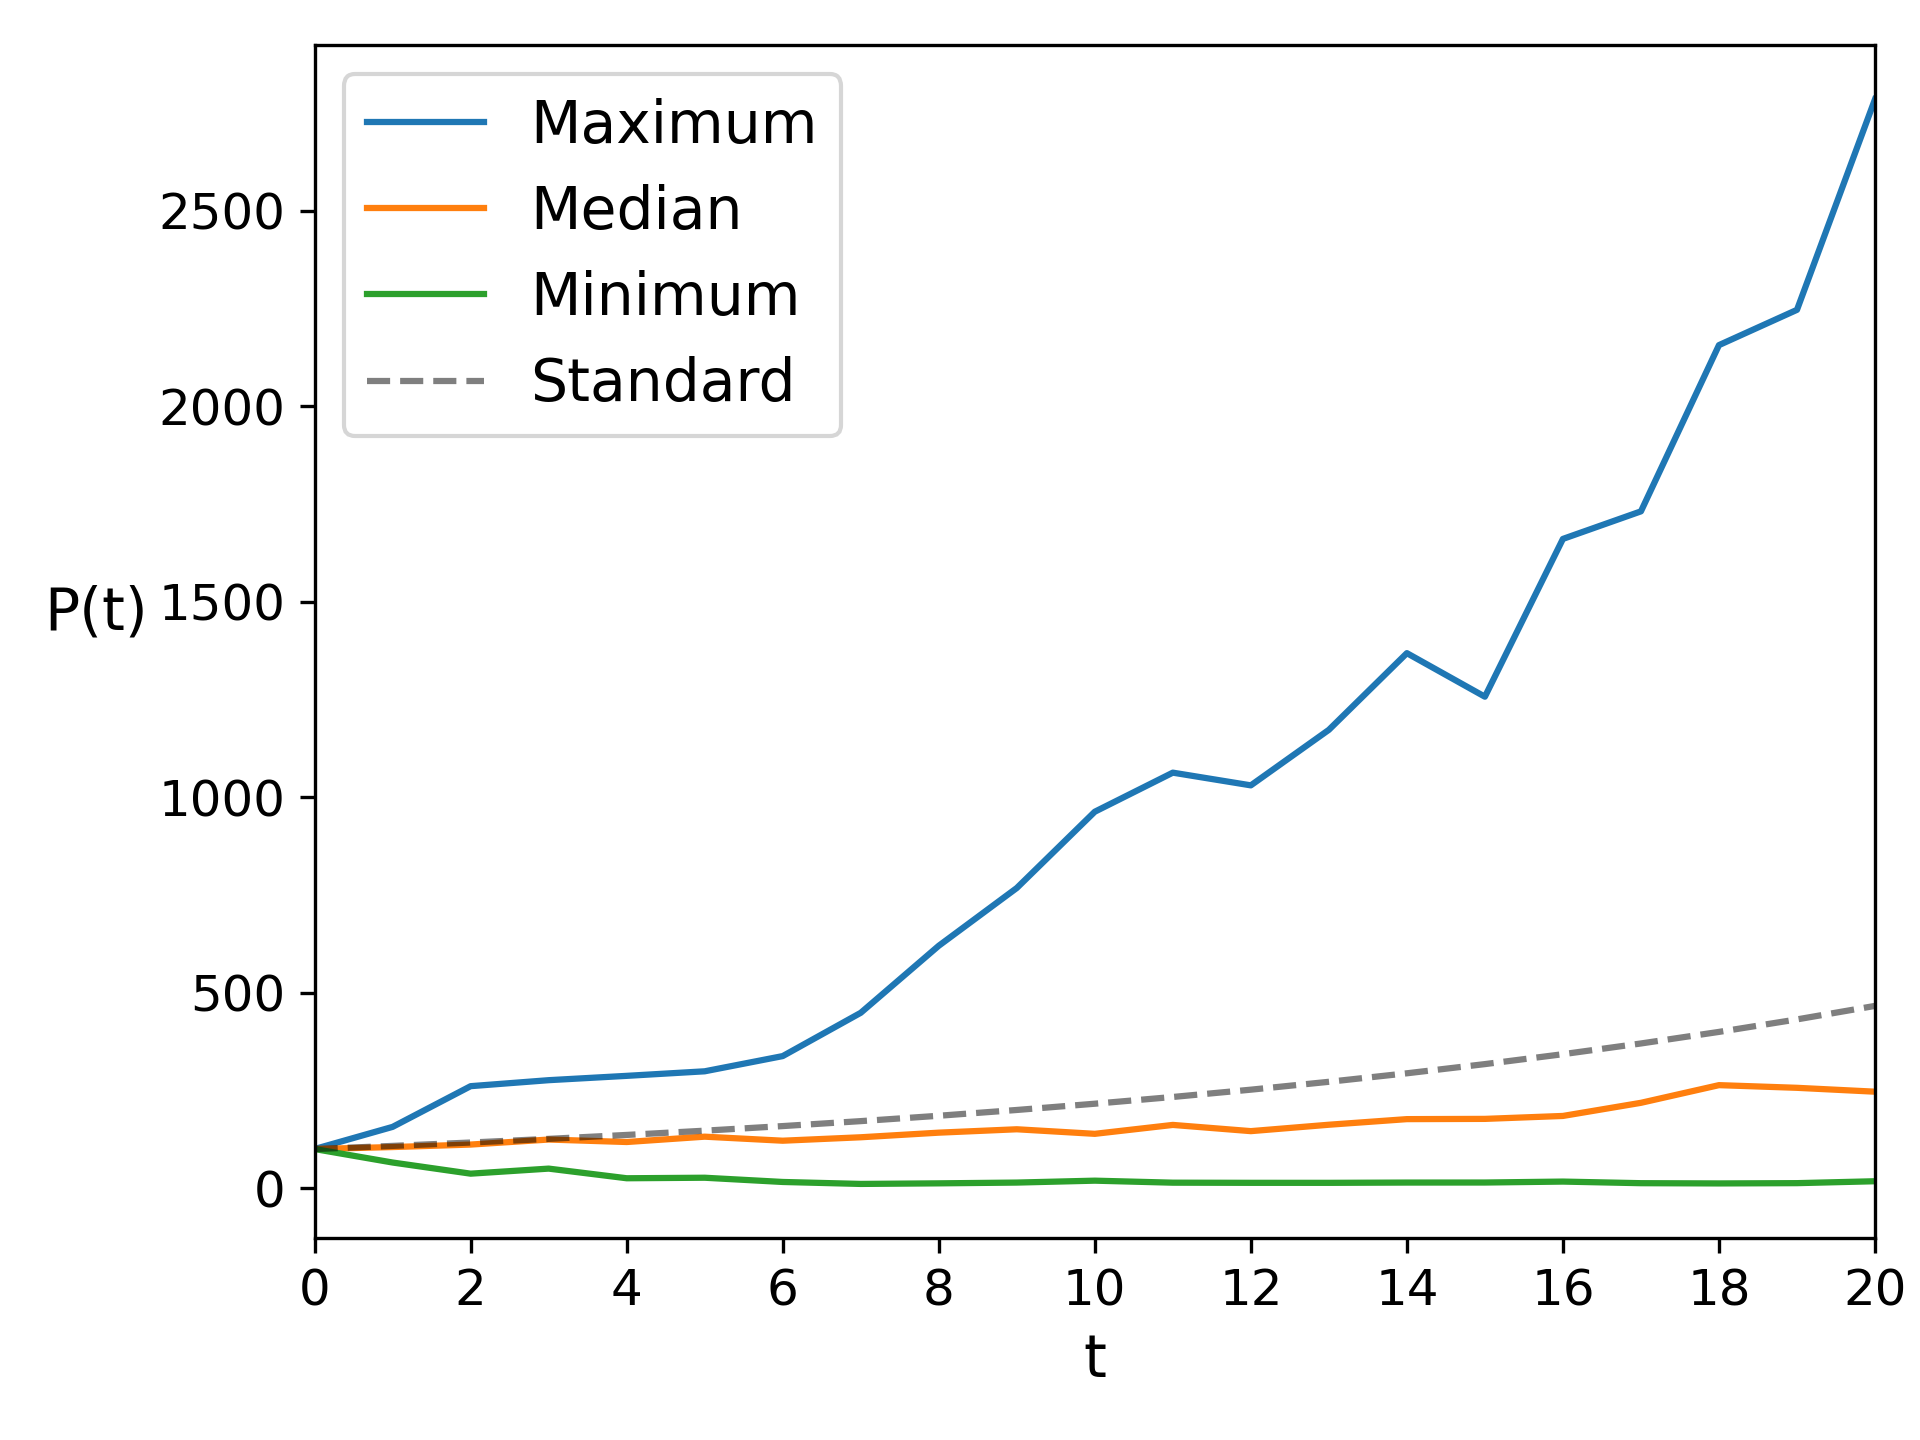
\includegraphics[width=.95\linewidth]{./plots/demographic_higher_dev.png}
        \caption{$b = \mathcal{N}(0.4,0.2)$ and $s = \mathcal{N}(0.68, 0.14)$}
        \label{fig:demographic-higher}
    \end{subfigure}
    \caption{Bobcat population over 20 years and 50 trail runs using different normal distributions for $b$ and $s$ parameters, with the standard exponential function as shown in \cref{fig:exponential} in gray.}
    \label{fig:demographic}
\end{figure}

In \cref{fig:demographic-standard} we see that our median stays fairly close to our initial exponential function. The maximum population function varies heavily from our median, while our minimum stays fairly close. This makes sense, our most common values will be in a single standard deviation, in birth rate this will be $0.4 \pm 0.1$, and in survival rate this will be $0.68 \pm 0.07$. Combining this into our $r + 1$ value from \cref{eq:exponential-basic}, we get $1.08 \pm 0.17$. So within one standard deviation $r$ will be between $0.25$ and $-0.09$. Thus, we will tend to have between a larger positive growth rate and a smaller negative growth rate. So, when we are on the positive side of our standard deviation we will grow more than when we are on the negative side of our standard deviation.

This model is quite sensitive to a change in this deviation, if we double the previous deviations, as we see in \cref{fig:demographic-higher}, our maximum goes significantly higher than before. This now changes our first deviation to have a birth rate $0.4 \pm 0.2$ and a survival rate $0.68 \pm 0.14$, or $r$ to be between $0.42$ and $-0.26$. With both a larger positive and negative growth rate we see our maximum grow faster, and our minimum approach zero, which it had not before in \cref{fig:demographic}.

One major change we see is that the median trends below the standard exponential function. This makes sense though, the median represents the ``middle of the road'' population. Say we have a very bad year, a growth rate of $1.42$, followed by a very bad year, a growth rate of $0.74$. We know that the growth rates compound over the years, so on the third year we would expect $1.42 \times 0.74 \times P(t-1)$, or a growth of $5.08\%$. While, our standard model with a fixed growth rate will have $1.08 \times 1.08 \times P(t-1)$, or a growth of $16.64\%$. In our previous model we would get $1.25 \times 0.91 \times P(t-1)$, or a growth of $13.75\%$. Thus, as our standard deviation grows, our median gets further, and in our case further negative, from the exponential model.


\section{Environmental Stochasticity}

\section{TBD}

\section{Conclusion}

\end{document}